\section{Marco teórico}
El marco teórico se divide en tres secciones: la primera describe el funcionamiento de los procesos dentro de un sistema operativo, y la segunda aborda la creación de procesos concurrentes y la tercera ahondará un poco en la creación de objetos aleatorios dentro de un sistema computarizado.

\subsection{Funcionamiento de los procesos dentro de un sistema operativo}
Como hemos mencionado anteriormente los procesos se pueden definir como programas que se ejecutan dentro de un sistema operativo.

Cabe mencionar que un proceso puede pasar por distintos estados durante su ejecución, algunos de estos estados son:
\begin{itemize}
    \item \textbf{Proceso nuevo:} Cuando un proceso es creado por algún medio este se encuentra en estado nuevo.
    \item \textbf{En ejecución:} Un proceso está en ejecución cuando la CPU se encuentra procesando información a su respecto en un instante determinado de tiempo.
    \item \textbf{En pausa:} cuando el proceso es suspendido temporalmente por el sistema operativo este se pone en pausa, a la espera de poder continuar su ejecución. (Estas pausas pueden llegar a durar muy pocos milisegundos).
    \item \textbf{Bloqueado:} se refiere a cuando un proceso está esperando que ocurra un evento externo, como la disponibilidad de un recurso. En este estado el proceso puede durar más tiempo que en una pausa e incluso puede no volver a ejecutarse.
    \item \textbf{Terminado:} Cuando todas las tareas relacionadas con un proceso se han completado este proceso se encuentra en estado terminado.
\end{itemize}

Podemos ver un gráfico del comportamiento de estos estados en la figura~\ref{fig:estadosDeProcesos}.

\begin{figure}[!ht]
    \centering
    \caption{Estados de los procesos}
    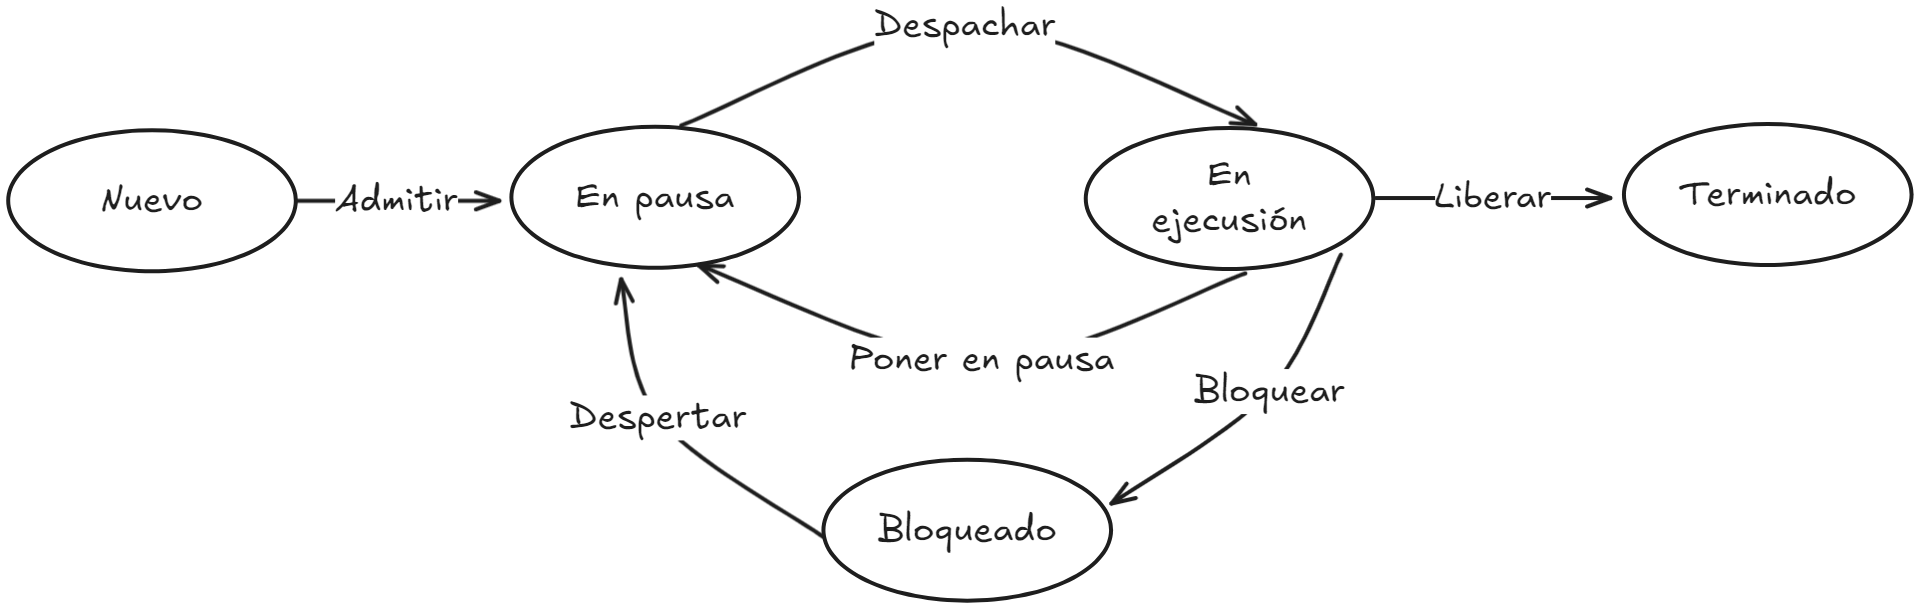
\includegraphics[width=0.9\textwidth]{src/images/Estados de procesos.png}\label{fig:estadosDeProcesos}
\end{figure}

Comprender los diferentes estados de un proceso así como el hecho de que al ejecutar en un mismo periodo varios procesos lo que ocurre realmente es que la CPU se encarga de ejecutar cada uno de ellos en un corto periodo en un orden determinado. (Como explicado en la introducción) es el fundamento del presente laboratorio.

\subsection{Creación de procesos concurrentes dentro de un sistema operativo}
Trabajar con procesos concurrentes dentro de un sistema operativo puede ser complejo si no se cuenta con los conocimientos necesarios para su creación y manejo.

Supongamos que, como se realizará posteriormente, tenemos tres programas encargados de la generación de productos de manera continua (números, letras, etc) y que deseamos ejecutarlos de manera paralela o, como se mencionará en adelante \textbf{de manera distendida}.

En caso de trabajar en un sistema Linux (como es el caso del presente laboratorio) para ejecutar los procesos en segundo plano, se puede usar el comando $\&$, lo que permite que el proceso continúe su ejecución mientras la consola queda disponible para otras tareas.

\begin{lstlisting}[language=bash, style=CodeStyle]
$ ./Generador_uno &
$ ./Generador_dos &
$ ./Generador_tres &
\end{lstlisting}

Esto indica que el proceso generador\_uno se ejecutará en segundo plano, lo mismo para el generador\_2 y para el generador\_tres. Al final de esta ejecución la consola quedará libre para poder continuar con otras tareas.

Para poder ver los procesos en ejecución y eliminarlos es necesario utilizar el comando \textit{ps} que nos devuelve una lista de todos los procesos en ejecución del sistema operativo.

\begin{lstlisting}[language=bash, style=CodeStyle]
$ ps
  PID TTY          TIME CMD
  101 pts/0    00:00:00 bash
  102 pts/0    00:00:00 ps
\end{lstlisting}

<<\textit{Si introduces el comando ps sin opciones, únicamente te mostrará los procesos iniciados por el shell actual. Por lo tanto, otros procesos quedan excluidos inicialmente.}>> \parencite{PS}.

Durante el presente informe se realizarán varios programas para su posterior ejecución mediante el uso del lenguaje C como veremos en el Procedimiento Experimental.

\subsection{Creación de números aleatorios}
<<\textit{Por naturaleza, las computadoras no son muy buenas con el azar. Su fortaleza radica en generar salidas predecibles ejecutando secuencias de operaciones programadas. Eso es casi lo opuesto a la aleatoriedad.}>> \parencite{NumerosAleatorios}.

De acuerdo con \textcite{eduardo2022Azar} el mejor método de generación de números aleatorios se encuentra en los sistemas cuánticos como el usado por la web \href{https://www.random.org/}{random.org}. Sin embargo no es muy cómodo tener que recurrir a información externa a un equipo para generar números aleatorios, por lo cuál se crearon con el tiempo algoritmos que generan números llamados \textbf{Pseudo Aleatorios}, es decir números que detrás llevan un desarrollo no aleatorio pero que a los ojos de los comsumidores lo son.

Una de las maneras de generar números de este tipo es mediante la técnica \textbf{LFSR} que se traduce al español como: \textit{registro de desplazamiento con retroalimentación lineal} que utiliza funciones lógicas sencillas y por tanto es muy sencilla de programar y de implementar a nivel del Hardware. El proceso consiste en lo siguiente:
\begin{enumerate}
  \item Se inicia con una semilla en binario.
  \item En cada repetición del proceso de cálculo se saca el último bit del número semilla.
  \item Posteriormente el resto de bits se corren a la derecha.
  \item En el espacio sobrante se agrega un bit, resultado de una operación lógica realizada sobre los bits restantes.
  \item Este proceso se repite, generando con los bits que se van retirando un número binario que se puede entregar como \"aleatorio\".
\end{enumerate}

Como se ve el procedimiento depende de la semilla usada; en caso de usar la misma semilla los resultados serán iguales, por lo que se precisa de una manera certera de crear semillas con las que alimentar este generador de pseudo-aleatoriedad.

Los diferentes lenguajes de programación tienen diferentes maneras de conseguir la semilla que será usada, como por ejemplo:
\begin{itemize}
  \item Usar el tiempo actual del sistema en el momento.
  \item Usar la cantidad de procesos activos en el sistema en el momento.
  \item Usar la cantidad de bytes libres en memoria en el momento.
  \item Usar el número del proceso en ejecución.
\end{itemize}